% !TEX encoding = UTF-8 Unicode

\documentclass[a4paper]{article}

\usepackage{color}
\usepackage{url}
\usepackage[T2A]{fontenc}
\usepackage[utf8]{inputenc}
\usepackage{graphicx}

\usepackage[english,serbian]{babel}


\usepackage[unicode]{hyperref}
\hypersetup{colorlinks,citecolor=green,filecolor=green,linkcolor=blue,urlcolor=blue}


\newtheorem{primer}{Primer}[section]

\begin{document}

\title{Hakovanje\\ \small{Seminarski rad u okviru kursa\\Računarstvo i društvo\\ Matematički fakultet}}

\author{Nikola Delić\\ nikoladelic9915@gmail.com}
\date{12.~maj 2022.}
\maketitle

\apstract{
Cilj ovog seminarkog rada je upoznavanje čitaoca sa istorijom i poreklom hakovanja, vrstama hakera koje postoje kao i nekim poznatijim hakerima kroz istoriju. Videćemo kako su se kroz istoriju razvijale tehnike sajber napada i količine štete koje su pravili. Bavićemo se i kaznama koje su dobijali ali i diskutovaćemo da li su njihove namere uvek bile zlonamerne.

\tableofcontents

\newpage

\section{Uvod}
\label{sec:uvod}
Hakovanje, koje vodi poreklo od nemačke reči u značenju "seći u komade", predstavlja proces obradjivanja informacija nakon čega dobijamo nešto korisno ili interesantno. Inicijalno je predstavljalo pozitivnu nameru, jer je na primer jedan od osnivača Apple-a Steve Wozniak smatran odličnim hakerom, ali se tada smatralo da je to osoba koja je vešta sa računarom i informacijama.
\newline
Medjutim danas, hakovanje više asocira na zlonamerno pronalaženje i otkrivanje kompjuterskih i mrežnih slabosti kako bi se one iskoristile za  krađu informacija, preuzimanje kontrole nad računarom i narušavanja privatnosti.
\newline
Naravno, ono nema uvek lošu konotaciju iz čega se javljaju razne vrste hakovanja.
}.

\newpage

\section{Istorijat}
Hakovanje se prvi put kao termin pojavljivao na sastancima Technical Model Railroad Club-a 1955-te gde se time smatralo visoko poznavanje računara i članovi kluba su hakovanjem zvali menjanje funkcija na višem nivou.
\newline
Tokom 60-ih godina obuhvatao je grupu računarskih entuzijanista. 1975-te, jedna od prihvaćenih definicija hakera od strane The Jargon File-a je bila: "Zlonamerni pojedinac koji pokušava da otkrije osetljive informacije koristeći svoje znanje iz informatike". To je bilo prvi put da je reč haker i hakovanje dato u sklopu sajber kriminala.
\newline
Prvim hakerom u istoriji smatra se John Draper poznatiji kao Captain Crunch. Nije koristio visokotehnološka sredstva već je sve radio sa igračkom zviždaljkom. Evo i kako je to radio: U to vreme, 70-ih godina, najveća računarska mreža je bila telefonski sistem. Telefonima je upravljao automatizovani sistem koji je koristio specifične  analogne frekvencije za upućivanje poziva. Draper je uspevao to da iskoristi koristeći igračku zviždaljku iz kutija žitarica. Ovo je radio za međugradske i internacionalne pozive. Tehnika je bila poznata pod nazivom "Phreaking".
\newline
Jedan od prvih internet hakera i sigurno prvih hakera koji je uspeo da privuče pažnju medija bio je Robert Moris 1989-te. Njegov napad izvršen je crvom koji je Moris razvio na Kornelskom univerzitetu. Moris tvrdi da nije hteo da nanese štetu vec da ukaže na sigurosne propuste ali je greška u kodu izazvala da se virus mnogo više širi i izazove štetu koja je trajala danima.
\newline
\newline
 \textbf{Vremenska linija istorije hakovanja:}
\begin{itemize}
\item 1971 - Draper je hakovao telefonski sistem i omogućio obavljanje besplatnih međugradskih i međunarodnih poziva
\item 1975 - Bill Gates i Paul Alen osnovali Microsoft
\item 1976 - osnivanje Apple kompjutera
\item 1989 - Morisov crv koji je usporavao rad procesora računara
\item 1990 - u Velikoj Britaniji se uvodi zakon kojim se bilo koji neautorizovani pristup računaru smatra ilegalnim
\item 1995 - kreiran je SSL da šifruje komunikaciju između kompjutera i udaljenog servera
\item 1999 - nastanak Windows-a 98 vodi ka tome da je sajber sigurnost postala uobičajena kod korisnika
\item 2000 - preko 10 miliona emajlova Windows korisnika biva inficiran Love bug-om,koji se najbrže širio u dotadasnjoj istoriji
\item 2002 - u Americi se sve vise priča o sajber kriminalu
\item 2003 - prva pojava Anonimusa i njihovih aktivnosti
\item 2008 - Anonimusi hakovali sajt Church of Scientology-a
\item 2010 - serija sajber napada pod nazivom Operacija Aurora 
\item 2013 - masovna provala Yahoo-a,dovelo do kompromitovanja 3 milijarde naloga
\item 2016 - Wikileaks

\end{itemize} 

\newpage


\section{Ko su hakeri?}	
\label{sec:naslov1}
Haker je osoba koja neovlašćeno pristupa računarima i računarskim mrežama.
\newline
Postoje tri vrste hakera: white hat, black hat i gray hat.
\subsection{White hat}
\label{subsec:podnaslov1}
White hat hakeri su hakeri koji hakuju radi poboljšanja sigurnosti sistema. Oni koriste takozvano etičko hakovanje\footnote{Etičko hakovanje je hakovanje čiji cilj nije zlonameran već predstavlja tip hakovanja koji pomažu programerima koji učestvuju u pravljenju sigurnosnih sistema.} kojim pronalaze propuste i greške u sigurnosnim kodovima i samim tim ukazuju na to koje stvari treba promeniti kod sistema kako bi on postao bezbedniji. Vrlo često koriste tehnike black hakera (o kojima će biti reč) kako bi obuhvatili sva scenarija koja se mogu desiti. Vrlo često su white hakeri nekada bili black hakeri, samim tim znaju sve načine na koji black haker moze ugroziti računar ili računarsku mrežu.
\newline
\newline
Neki od poznatijih White hakera:
\begin{itemize}
	\item Marc Maiffret - radio na otkrivanju ranjivosti Microsoft proizvoda,kao sto je npr Code Red worm
	\item Kevin Mitnic - 1995-te bio jedan od najtraženijih sajber kriminalaca u SAD zbog svojih hakerskih radnji, uhapšen i služio kaznu od 5 godina, nakon koje je postao white hacker i pomagao vladi
	\item Robert "Rsnake" Hansen - bio osnivač kompanije za borbu protiv ilegalnih radnji na kompjuteru
\end{itemize}
\subsection{Black hat}
\label{subsec:podnaslov2}
Zlonamerni hakeri čiji je jedini cilj lična dobit ili sabotaža sistema.
\newline
Neki od poznatijih black hat hakera:
\begin{itemize}
	\item Kevin Mitnick
	\item Anonymous
	\item Adrian Lamo
	\item Albert Gonzales
	\item Matthew Bevan i Richard Pryce
	\item Jeanson James Anceta
	\item Michael Calce
	\item Kevin Poulsen
	\item Jonathan James
	\item Astra
\end{itemize}
O nekima ce biti reč kasnije.
\subsection{Grey hat}
Nemaju zle namere ali žele da provale u sistem treće strane.
\subsection{Script Kiddie}
Ljudi koji žele da hakuju kako bi nešto naučili.
\newpage



\section{Najpoznatiji hakeri}
\label{hakeri}

\subsection{Anonymous}
Anonymous je počeo sa radom 2003. godine na 4chanu na neimenovanom forumu. 2008. godine suočili su se sa Churc - om of Scientology i počeli da obaraju njihove stranice, što je onemogućilo njihovo pretraživanje na Googl-u. Njihove fax mašine su bile preplavljenje crnim slikama. U martu iste godine grupa "Anona" marširala je pored tog centra noseći sad već čuvenu masku  Guy Fawksa. Policija u New Yorku je ušla u trag nekim jačim članovima grupe ali je zbog toga što ne postoji hijerarhija u ovoj organizaciji veoma teško pronaći sve članove.





\begin{figure}[h!]
\begin{center}
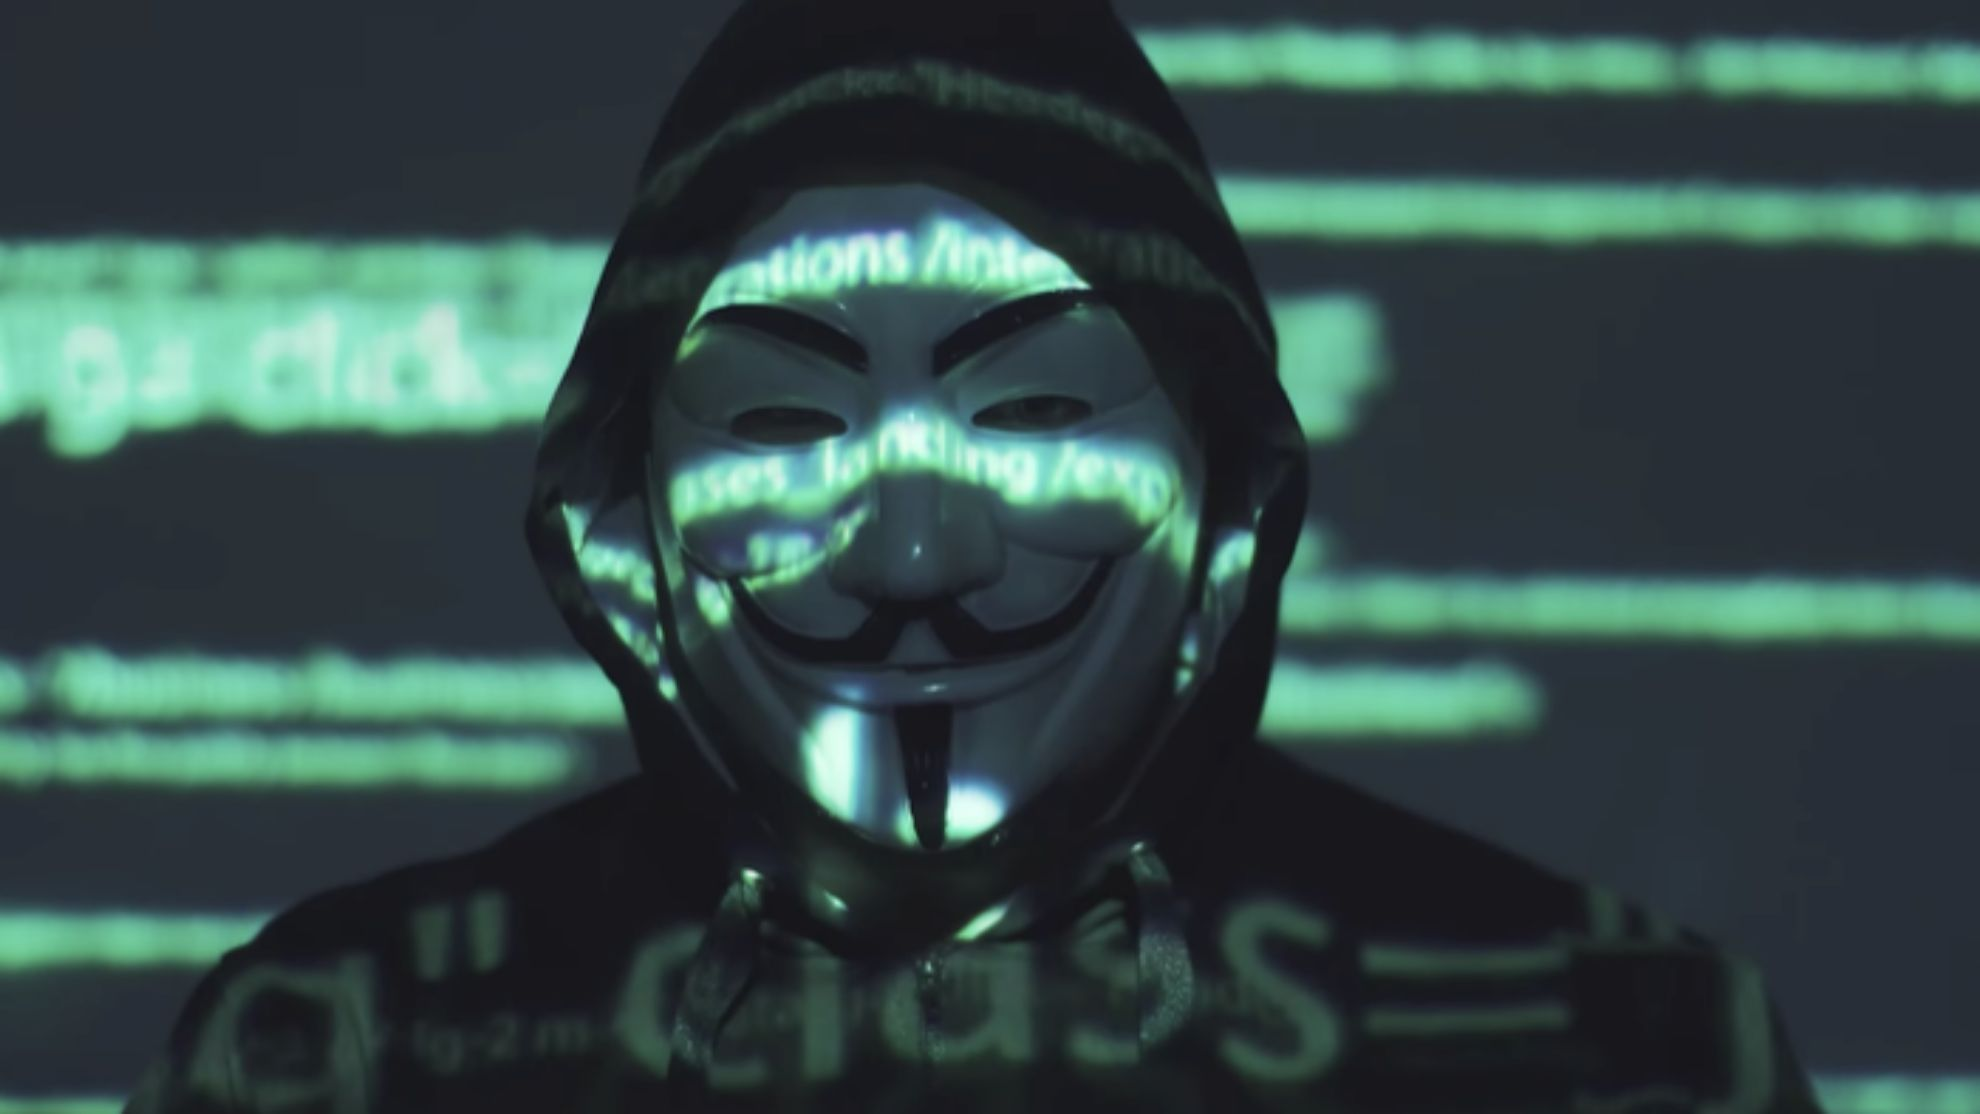
\includegraphics[scale=0.10]{anonymous.jpg}
\end{center}
\caption{Anonymous}
\label{fig:anonymous}
\end{figure}

 Na slici \ref{fig:anonymous} prikazana je maska Anonymusa. 
 
 \subsection{Adrian Lamo}
Godine 2001, 20-to godišnji Adrian Lamo koristio je nezaštićen alat za upravljanje sadržajem na Yahoo da modifikuje Rojtersove članke i doda lažni citat koji se pripisuje bivšem državnom tužiocu Dzonu Ashcroft-u. često je hakovao sisteme a zatim o tome obaveštavao medije i žrtvu. U nekim slučajevima je pomagao žrtvama čišćeći njihove sisteme i poboljšavajući zaštitu. Prešao je granicu kada je 2002. godine editovao New York Times i sebe stavio kao istraživača. Bio je poznat pod nazivom "Haker beskućnik" jer je često lutao ulicama sa samo rancem i nije imao stalnu adresu.
\begin{figure}[h!]
	\begin{center}
		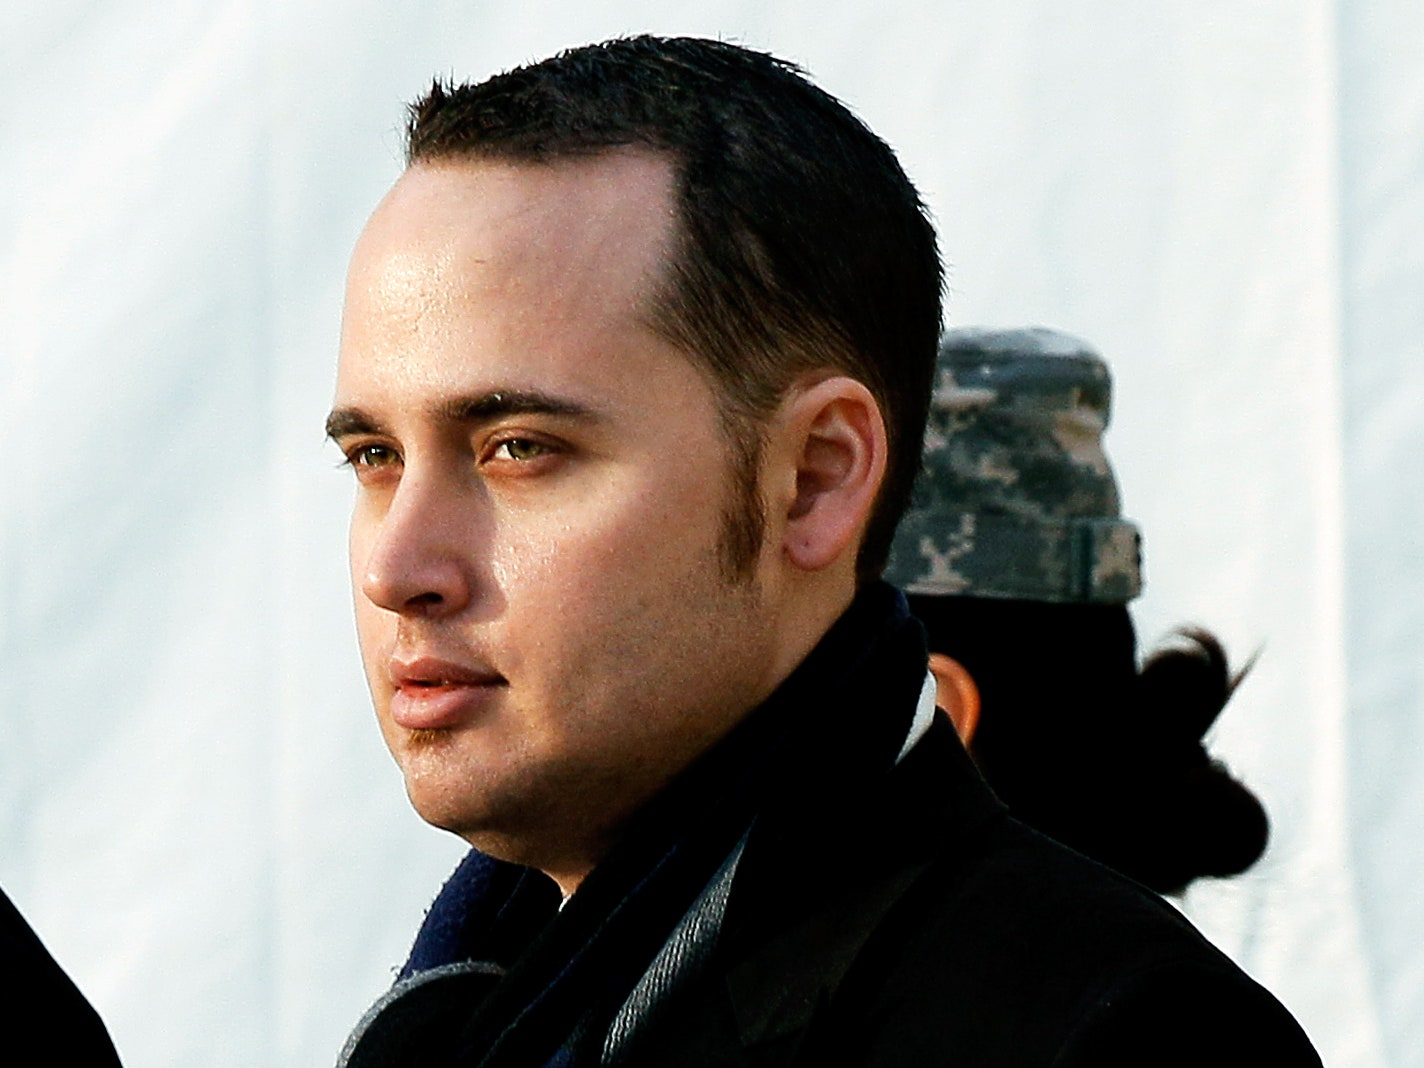
\includegraphics[scale=0.10]{adrian.jpg}
	\end{center}
	\caption{Adrian}
	\label{fig:adrian}
\end{figure}

Na slici \ref{fig:adrian} je Adrian Lamo.

\newpage
\subsection{Albert Gonzales}
Albert Gonzales zvani "soupnazi" počeo je kao "problematični vođa grupe kompjuterskih štrebera" u srednjoj školi u Majamiju. Kasnije je počeo da bude aktivan na kriminalnom trgovinskom sajtu Shadowcrew.com i bio smatran jednim od njihovih najboljih hakera. Sa 22 godine je bio uhapšen u Njujorku zbog sumnje da je izvršio krađu sa preko milion debitnih kartica. Da bi izbegao zatvor, postao je doušnik Tajnoj sluzbi u pronalaženju ostalih članova Shadowcrew-a. Dok je pomagao Tajnoj službi, i dalje se bavio prevarama i krađom podataka sa kartica.
\begin{figure}[h!]
	\begin{center}
		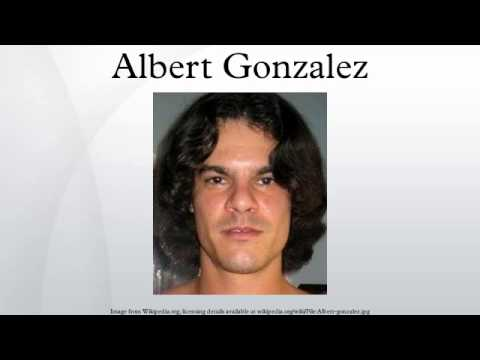
\includegraphics[scale=0.25]{albert.jpg}
	\end{center}
	\caption{Albert}
	\label{fig:albert}
\end{figure}

Na slici \ref{fig:adrian} je Albert Gonzales.
\subsection{Jeanson James Ancheta}
Jeanson James Ancheta nije bio zainteresovan u krađi sa debitnih kartica ili rušenju računarskih mreža. Umesto toga, zanimao se botovima-softver robotima kako bi zarazio i kontrolisao računarske sisteme. Koristeći veliki broj botova uspeo je da ugrozi preko 400 000 računara. Bio je osuđen na 57 meseci zatvora. Ovo je bio prvi slučaj da je haker dobio zatvorsku kaznu zbog korišćenja botnet tehnologije.
\begin{figure}[h!]
	\begin{center}
		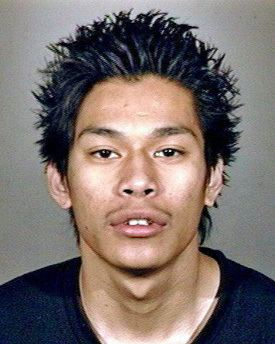
\includegraphics[scale=0.30]{james.jpg}
	\end{center}
	\caption{James}
	\label{fig:james}
\end{figure}

Na slici \ref{fig:james} je Jeanson James Ancheta.
\newpage

\subsection{Michael Calce}
U februaru 2000. godine, 15-to godišnji Michael Calse poznatiji kao "Mafiaboy", uspeo je da zauzme sve mreže univerzitetskih računara. Koristio je te resurse kako bi oborio glavni pretraživac u to vreme Yahoo. Za nedelju dana, takođe je uspeo da obori Dell, eBay, CNN i Amazon. Njegov hakerski napad uticao je mnogo na razvoj zakona o sajber kriminalu jer ako su ovako velike kompanije mogle tako lako da padnu, šta bi onda bilo sa manje zaštićenim podacima. Ubrzo je sajber kriminal postao jedna od glavnih tema vlade zahvaljujući napadu Michael Calce-a.
\begin{figure}[h!]
	\begin{center}
		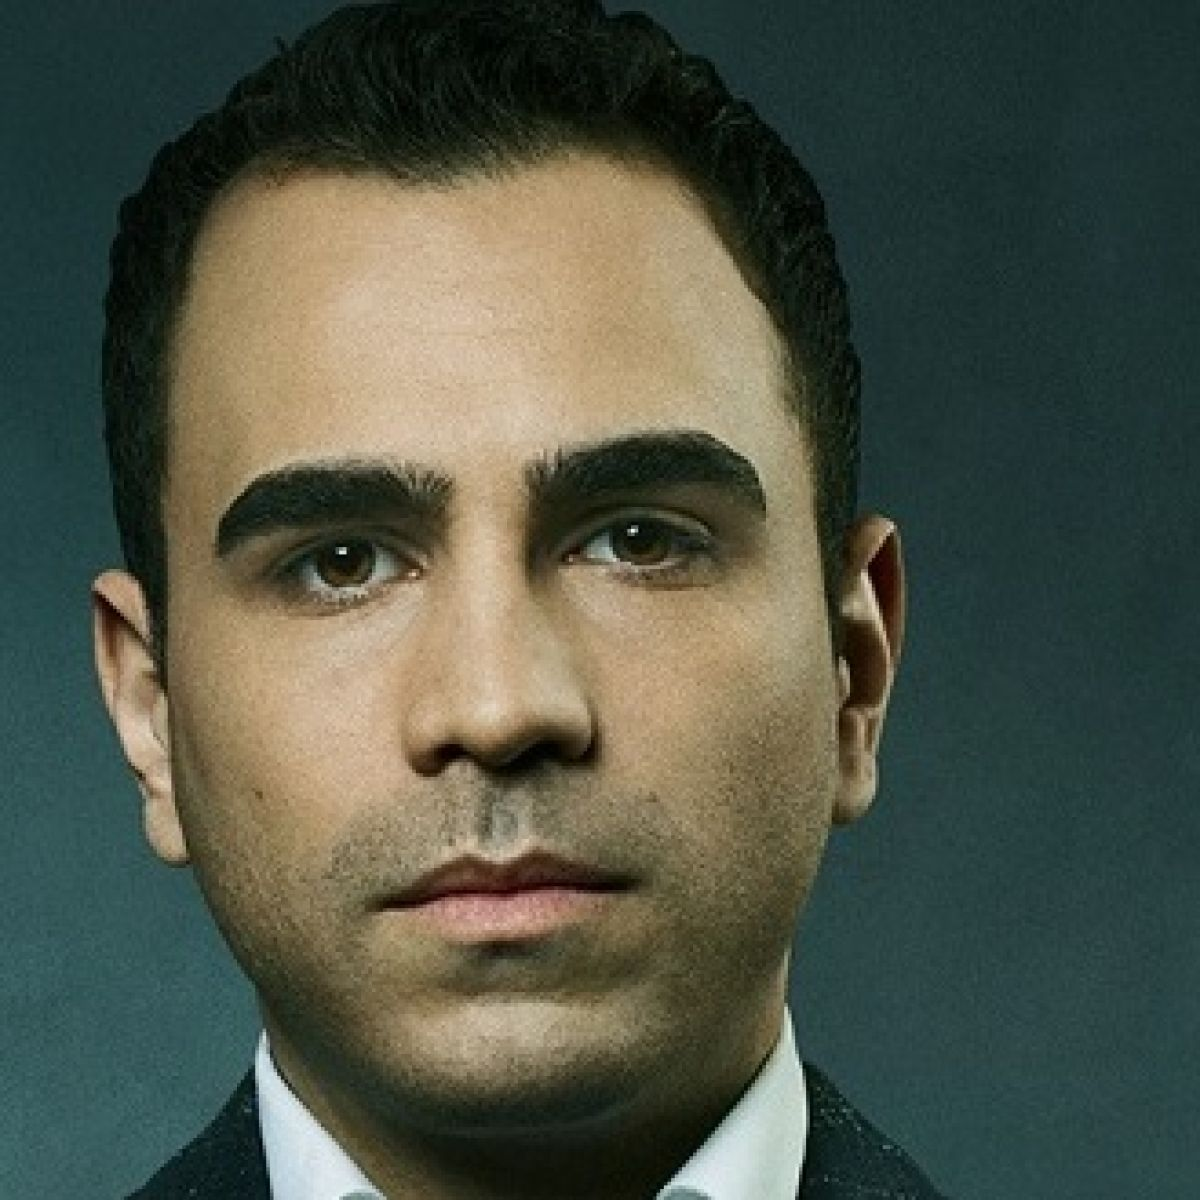
\includegraphics[scale=0.10]{michael.jpg}
	\end{center}
	\caption{Michael}
	\label{fig:michael}
\end{figure}

Na slici \ref{fig:michael} je Michael Calce.
\subsection{Astra}
Ovaj haker se razlikuje od ostalih na listi jer nikada nije javno identifikovan. Međutim, postoje neki nepotvrđeni podaci koji govore o tome da je uhapšen 2008. godine i da se radi o 58-mo godišnjem grčkom matematičaru. Krao je podatke o oružju i prodavao određenim pojedincima. Njegov identitet nikada nije otkriven ali se zna da reč "astra" označava oružje.
\begin{figure}[h!]
	\begin{center}
		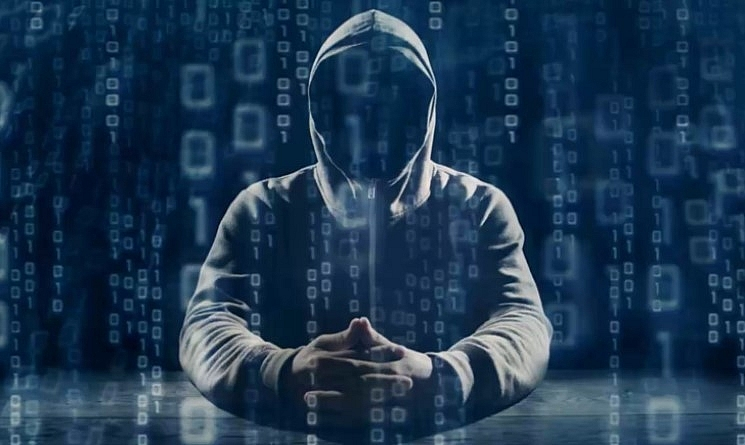
\includegraphics[scale=0.20]{astra.jpg}
	\end{center}
	\caption{Astra}
	\label{fig:astra}
\end{figure}
\newpage
\section{Kazne za hakere}
\label{kazne}
Kazne za hakere regulisane su u okviru Krivičnog zakona Republike Srbije.Obuhvaćene su u okviru tri člana:302,303,304.
\subsection{Član 302: Neovlašćeni pristup zaštićenom računaru,računarskoj mreži ili elektronskoj obradi podataka}
\begin{itemize}
	\item Ko se,kršeći mere zaštite neovlašćeno uključi u računar ili računarsku mrežu ili neovlašćeno pristupi elektronskoj obradi podataka, kazniće se novčanom kaznom ili zatvorom do šest meseci.
	\item Ko upotrebi podatak dobijen na način predviđen u stavu 1 ovog člana, kazniće se novčanom kaznom ili zatvorom do dve godine.
	\item Ako su usled dela iz stava 1. ovog člana došlo do zastoja ili ozbiljnog poremećaja funkcionisanja elektronske obrade i prenosa podataka ili mreže ili su nastupile druge teške posledice, učinilac će se kazniti zatvorom do tri godine.
\end{itemize}
\subsection{Član 303: Sprečavanje i ograničavanje pristupa javnoj računarskoj mreži}
\begin{itemize}
	\item Ko neovlašćeno sprečava ili ometa pristup javnoj računarskoj mreži, kazniće se novčanom kaznom ili zatvorom do jedne godine
	\item Ako delo iz stava 1 ovog člana učini službeno lice u vršenju službe, kazniće se zatvorom do tri godine.
\end{itemize}
\subsection{Član 304: Neovlašćeno korišćenje računara ili računarske mreže}
\begin{itemize}
	\item Ko neovlašćeno koristi računarske usluge ili računarsku mrežu u nameri da sebi ili drugom pribavi protivpravnu imovinsku korist, kazniće se novčanom kaznom ili zatvorom do tri meseca.
	\item Gonjenje za delo iz stava 1. ovog člana preduzima se po privatnoj tužbi.
\end{itemize}
\begin{figure}[h!]
	\begin{center}
		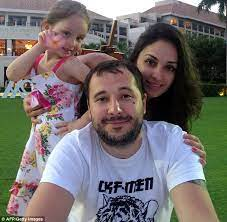
\includegraphics[scale=0.30]{roman.jpeg}
	\end{center}
	\caption{Roman Seleznev,haker koji je osuđen na najveću kaznu,27 godina zatvora}
	\label{fig:roman}
\end{figure}
\newpage









 

\section{Zaključak}
\label{sec:zakljucak}
Od nastanka računarstva i kompjuterske tehnologije postoje hakerske delatnosti. Daljim razvojem softvera i mogućnosti razvijale su se i različite vrste hakovanja i napada na računarske sisteme. Moramo biti svesni da se svi naši podaci nalaze na internetu i da je uzaludno govoriti o nekoj vrsti privatnosti.U takvoj situaciji,vrlo lako postajemo žrtve sajber napada i jako teško možemo da se odbranimo od istih.Videli smo da su u mogućnosti da naprave milionske štete i da pritom često izbegnu neku veću zatvorsku kaznu.
\newline
Međutim, ne treba stvari posmatrati samo na taj način. Hakeri su poprimili većinom negativnu konotaciju ali moramo shvatiti da su upravo oni ti koji su tu da nas upozore da nam privatnost može biti narušena. Njihov motiv je često čista želja za unapređenjem svog znanja i veština a ne samo krađa i zloupotreba podataka. Vrlo često to rade iz čistog osećaja zadovoljstva kada uspeju da probiju neki računarski sistem. Vrlo često su i sami borci za pravdu i slobodu. Mnogi od njih poseduju određene kodekse i etičke norme čime ne predstavljaju nikakvu opasnost. Zato treba gledati na njih i iz drugog ugla,i probati nešto naučiti.
 

\newpage


\addcontentsline{toc}{section}{Literatura}
\appendix

\iffalse
\bibliography{seminarski} 
\bibliographystyle{plain}
\fi

\begin{thebibliography}{9}

\bibitem{history} https://cybernews.com/security/brief-history-of-cybersecurity-and-hacking/

\bibitem{history} https://www.helpnetsecurity.com/2002/04/08/the-history-of-hacking/

\bibitem{whitehat} https://www.kaspersky.com/resource-center/definitions/white-hat-hackers

\bibitem{blackhat} https://www.kaspersky.com/resource-center/threats/black-hat-hacker

\bibitem{hackers}  https://www.kaspersky.com/resource-center/threats/top-ten-greatest-hackers

\bibitem{prez} prezentacija-bezbednost na internetu


\end{thebibliography}




\appendix



\end{document}
